% !TeX spellcheck = pt_BR
\chapter[Semana 1]{}
\chaptermark{}


\hfill%
\begin{minipage}{10cm}
\begin{flushright}
\rightskip=0.5cm
\textit{``You know also that the beginning is the most important part of any work''}
\\[0.1cm]
\rightskip=0.5cm
---Plato's Republic
\end{flushright}
\end{minipage}


\section{Introdução}

O conjunto dos números complexos $\mathbb{C}$
pode ser construído de diversas maneiras.
Algumas destas construções adotam abordagens puramente algébricas,
enquanto outras são um pouco mais geométricas. O objetivo desta seção 
é apresentar três alternativas para se construir o conjunto dos números complexos. 

Sem dúvida, entre todas as construções conhecidas a mais simples (porém abstrata) é aquela que introduz 
o conjunto dos número complexos como um conjunto abstrato de símbolos munido de duas operações binárias (soma e produto). 
Seus elementos são simplesmente símbolos da forma $a+ib$, onde $a$ e $b$ podem ser quaisquer números reais 
e a letra ``$i$\,'' é simplesmente um símbolo especial que será chamado de 
unidade imaginária.\index{Unidade imaginária} 
Por exemplo, $1+i\pi$ é um elemento deste conjunto. Mas como nada foi dito ainda sobre as operações algébricas, 
por enquanto o símbolo $1+i\pi$ só tem o significado de ser um amontoado 
4 caracteres escritos numa ordem especial. Em particular, nesta notação, apesar de sugerir, 
o símbolo ``$+$'' ainda não tem significado de uma soma e nem o símbolo $i\pi$
de um produto. Poderíamos prosseguir com a brincadeira 
(sem graça e aparentemente sem sentido) de listar mais elementos deste conjunto, escrevendo por exemplo símbolos como
$7+i3$ ou $\frac{1}{2}+i9$ e assim por diante. 
Claramente, nada de interessante apareceria disto e muito menos claro ainda seria qual a 
relação deste conjunto com a ideia intuitiva de que já temos do que sejam números. 

As responsáveis por estabelecer a relação entre o conjunto dos símbolos da forma $a+ib$ e a ideia de números 
são as operações algébricas de soma e produto definidas abaixo:
\begin{itemize}
\item $(a+ib)+(c+id) = (a+c)+i(b+d)$
\item $(a+ib)\cdot (c+id) = (ac-bd)+i(ad+bc)$.
\end{itemize}

Vamos ver agora um pouco do porquê a introdução destas operações dá vida 
à notação que usamos
para apresentar o conjunto $\mathbb{C}$. 
Primeiro observe que se identificamos um elemento da forma $a+i0$ 
com o número real $a$, então podemos pensar que as operações 
definidas acima são extensões das operações usuais de soma e produto de números reais. 
Isto é, a soma dos números complexos identificados com os números reais $a$ e $c$ é dada por 
$(a+i0)+(c+i0)=(a+c)+i0$ e portanto identificada com o número real $a+c$. Analogamente, 
o produto dos números complexos identificados com os números reais $a$ e $c$, é dado pela expressão
$(a+i0)\cdot(c+i0)=ac+i0$ que por sua vez é identificada com o número real $ac$. 

Da forma como foram definidas as operações em $\mathbb{C}$
somos levados naturalmente a identificar a unidade imaginária $i$ com o 
número complexo $0+i1$. Consequentemente, temos a relação
$i^2 = i\cdot i = (0+i1)\cdot(0+i1)= -1+0i = -1$. 
Desta simples observação podemos concluir que existe pelo menos 
um número complexo $z=a+ib\in \mathbb{C}$ 
que resolve a equação $z^2+1=0$. Este fato enfatiza a importância 
da unidade imaginária dentro do conjunto $\mathbb{C}$, já que não existe nenhum número 
real $x$ tal que $x^2+1=0$. Seguindo, vemos que a definição de produto nos permite interpretar 
o símbolo $ib$ em $a+ib$ como um produto da unidade imaginária pelo número real $b$. 
Para isto usamos primeiros as identificações mencionadas acima, em seguida que  
$i\cdot b = (0+i1)(b+0i)=0+ib$ e por último identificamos $0+ib$ com $ib$ obtendo 
a interpretação desejada. 
O leitor mais atento deve ter observado que até este momento fomos cuidadosos com a ordem dos termos da
nossa notação. Vamos voltar a este assunto mais a frente. 

%Mas a verdade é que usando as identificações já mencionadas e as operações 
%definidas acima, podemos verificar, por exemplo, que $i\cdot d$ e $d\cdot i$ representam o mesmo 
%número complexo. De fato, $i\cdot d = (0+i1)(d+i0) = 0+id = (d+i0)(0+id) = d\cdot i$.
%Mais geralmente, dados quaisquer números complexos $a+ib$ e $c+id$ temos que  
%Consequentemente, podemos olhar para 

Com o exposto até aqui já podemos imaginar como proceder para extrair
as demais propriedades algébricas básicas dos números complexos.
Por outro lado, uma boa parcela dos leitores deve ter ficado com a sensação de que esta é uma 
construção muito abstrata e um tanto quanto artificial. Para remediar isto, vamos
apresentar, em seguida, outra construção de caráter também algébrico, porém feita a partir de objetos matemáticos
bem mais familiares, matrizes! 

\bigskip 


Antes de prosseguir observamos que independentemente de como seja construído o conjunto dos números 
complexos nele sempre devem existir três elementos muito especiais: 
\begin{itemize}
	\item uma unidade imaginária, tradicionalmente denotada por $i$;
	\item um elemento neutro para a operação de produto, frequentemente denotado por $1$ ou $\mathds{1}$; 
	\item um elemento neutro para a operação de soma, frequentemente denotado pelo símbolo $0$.
\end{itemize}
Além do mais, é fundamental, em qualquer que seja a construção, que a seguinte
propriedade seja válida:
\\[0.3cm]
(P1) - o quadrado da unidade imaginária (quadrado com relação ao produto definido) somado ao elemento neutro do produto
de ser igual ao elemento neutro da soma. 
\\[0.3cm]

A fim de apresentar uma nova construção do conjunto dos números complexos 
satisfazendo a propriedade (P1) vamos explorar o espaço de matrizes. A exposição feita aqui é semelhante
à apresentada na referência \cite{MSoa16}. 
A princípio esta estratégia poderia soar um pouco estranha, mas a verdade é que o conjunto 
de matrizes com suas operações usuais é uma das poucas estruturas algébricas fora da lista
$\mathbb{N}$, $\mathbb{Z}$, $\mathbb{Q}$ e $\mathbb{R}$ que conhecemos quando estamos começando a estudar
matemática.

Como já mencionamos, certos espaços de matrizes já possuem estruturas naturais 
de soma e produto e assim parte das tarefas
da construção (que consiste em apresentar as propriedades algébricas) já estariam realizadas.
Por questão de simplicidade, é mais prudente iniciar nossa exploração pelo mundo das matrizes $2\times 2$ com entradas reais.
É claro que mais simples ainda seria começar pelas matrizes $1\times 1$ com entradas reais, 
porém este espaço com suas operações usuais é idêntico (do ponto de vista algébrico) ao 
conjunto dos números reais. Desta forma não seria possível 
escolher nenhum elemento dentro deste conjunto para fazer o papel da unidade imaginária de 
forma que a propriedade (P1), nele, fosse satisfeita.

Denote por $\mathbb{M}_{2\times 2}(\mathbb{R})$ o conjunto de todas as matrizes $2\times 2$ com entradas reais.
Vamos adotar as notações $\mathds{1}$ e $0$ para denotar, respectivamente, as matrizes: identidade e nula em $\mathbb{M}_{2\times 2}(\mathbb{R})$. Isto é, 
\[
\mathds{1}
\equiv
\begin{pmatrix}
1&0\\
0&1
\end{pmatrix} 
\qquad\text{e}\qquad 
0 
\equiv
\begin{pmatrix}
0&0\\
0&0
\end{pmatrix}.  
\]
Lembre-se que $\mathds{1}$ é o elemento neutro da operação usual de produto em $\mathbb{M}_{2\times 2}(\mathbb{R})$
e $0$ é o elemento neutro da soma, neste conjunto. 
Portanto, perguntar se a propriedade (P1) é satisfeita
em $\mathbb{M}_{2\times 2}(\mathbb{R})$ é equivalente a perguntar se existe
alguma matriz $X\in \mathbb{M}_{2\times 2}(\mathbb{R})$ satisfazendo 
\[
X\cdot X +\mathds{1} =0
\qquad \text{equivalentemente} \qquad 
X^2+\mathds{1}= 0.
\]
Se tal matriz existir ela é candidata natural para representar a unidade imaginária. 

Para resolver a equação acima, precisamos verificar se existem $x,y,z,w\in\mathbb{R}$ tais que 
\[
\begin{pmatrix}
x&y\\
z&w
\end{pmatrix}
\cdot
\begin{pmatrix}
x&y\\
z&w
\end{pmatrix}
+
\begin{pmatrix}
1&0\\
0&1
\end{pmatrix}
=
\begin{pmatrix}
0&0\\
0&0
\end{pmatrix}.
\] 
Com um pouco de paciência e utilizando o velho método de tentativa e erro, descobrimos rapidamente que 
o problema acima admite a solução $x=0$, $y=-1$, $z=1$ e $w=0$. Desta forma temos um candidato a unidade 
imaginária, que respeitando a tradição será denotado por
\[
i
=
\begin{pmatrix}
0&-1\\
1&0
\end{pmatrix}.
\]

Apesar da propriedade (P1) ser satisfeita em $\mathbb{M}_{2\times 2}(\mathbb{R})$, não podemos
usar o espaço como um todo para construir o conjunto $\mathbb{C}$. Uma das razões, que não mencionamos anteriormente, 
é que independentemente de como construímos $\mathbb{C}$ a operação de produto deve ser comutativa.
Por outro lado, é bem conhecido que a operação de produto em $\mathbb{M}_{2\times 2}(\mathbb{R})$ não é comutativa. 
Apesar desta nossa tentativa inicial ter sido frustrada rapidamente por esta obstrução, 
restaria ainda a esperança de se prosseguir
com a construção considerando um subconjunto próprio de $\mathbb{M}_{2\times 2}(\mathbb{R})$ 
em que a operação de produto fosse comutativa. 
Adotando esta estratégia a primeira coisa que viria em mente é restringir nossa atenção apenas ao subconjunto 
das matrizes diagonais em $\mathbb{M}_{2\times 2}(\mathbb{R})$, pois sabemos que a multiplicação de matrizes restritas 
a este subconjunto é certamente comutativa. 
Mas, infelizmente, isto nos causaria outro problema. A candidata à unidade imaginária, 
construída acima, não é um elemento do conjunto das matrizes diagonais. 
Já que a candidata a unidade imaginária proposta acima foi construída pelo método de erro e tentativa,  
poderíamos voltar à equação $X^2+\mathds{1}=0$ e verificar 
se seria possível encontrar uma matriz diagonal em $\mathbb{M}_{2\times 2}(\mathbb{R})$ 
que resolvesse este problema. Após alguns poucos cálculos descobriríamos que nenhuma matriz 
diagonal em $\mathbb{M}_{2\times 2}(\mathbb{R})$ pode ser uma solução desta equação.


Para continuar nossa busca precisamos investigar se existem outros 
subconjuntos de $\mathbb{M}_{2\times 2}(\mathbb{R})$ que além de possuir a nossa já construída unidade imaginária 
seja tal que a operação de produto restrita a ele é comutativa. 
Isto nos leva naturalmente a considerar a seguinte pergunta. 
\\
{\bf Pergunta.} Existe algum subconjunto de 
$\mathscr{C}\subset \mathbb{M}_{2\times 2}(\mathbb{R})$ possuindo a nossa candidata à unidade imaginária e também satisfazendo a seguinte propriedade: para quaisquer $A,B\in \mathscr{C}$ temos 
$A\cdot B = B\cdot A$? 

Uma maneira de atacar este problema é começar construindo uma coleção matrizes, a mais simples possível, 
de forma que todos os elementos deste conjunto comutem entre si e também com a matriz
\[
i= 
\begin{pmatrix}
0&-1\\
1&0
\end{pmatrix}.
\]

Para isto vamos usar o fato bem conhecido de que a matriz identidade $\mathds{1}$ comuta com qualquer
matriz e em particular com a matriz $i$. Na verdade, para todo $a\in\mathbb{R}$ 
temos que a matriz 
\[
a\mathds{1} 
= 
\begin{pmatrix}
a&0\\
0&a
\end{pmatrix}
\] 
comuta com a matriz $i$. De forma mais geral, dados quaisquer $a,b\in\mathbb{R}$
temos que as matrizes
\[
a\mathds{1} 
= 
\begin{pmatrix}
a&0\\
0&a
\end{pmatrix}
\qquad \text{e}\qquad 
bi= 
\begin{pmatrix}
0&-b\\
b&0
\end{pmatrix}
\]
comutam. 

Antes de prosseguir aproveitamos para observar que este é um bom momento 
para falarmos sobre a operação de soma, que permaneceu por um tempo 
esquecida da nossa discussão. O que queremos dizer é que em qualquer construção de $\mathbb{C}$
a soma de quaisquer dois elementos deste conjunto deve também ser um elemento deste conjunto. 
Desta forma nossa construção dos números complexos precisa possuir o elemento 
\[
a\mathds{1}+b i = 
\begin{pmatrix}
a&0\\
0&a
\end{pmatrix}
+
\begin{pmatrix}
0&-b\\
b&0
\end{pmatrix}
=
\begin{pmatrix}
a&-b\\
b&a
\end{pmatrix}.
\]
Isto nos motiva a propor o seguinte conjunto de $\mathbb{M}_{2\times 2}(\mathbb{R})$ 
como uma construção do conjunto dos números complexos
\[
\mathbb{C}
= 
\left\{
\begin{pmatrix}
a&-b\\
b&a
\end{pmatrix}
:
a,b\in \mathbb{R}
\right\}.
\] 

Várias propriedades exigidas de uma construção do conjunto dos números complexos já 
foram verificadas para este conjunto. Seguindo nossas notações uma matriz arbitrária 
pertencente ao nosso conjunto $\mathbb{C}$ pode ser escrita 
como $a\mathds{1}+ bi$ onde $a,b\in\mathbb{R}$.

Uma outra propriedade importante que ainda não mencionamos sobre a construção de $\mathbb{C}$
é que todo elemento não-nulo deve possuir um inverso multiplicativo. 
Isto é, para todo $a\mathds{1}+ bi$ em $\mathbb{C}$ deve existir um elemento $c\mathds{1}+ di$ em $\mathbb{C}$
tal que $(a\mathds{1}+ bi)\cdot (c\mathds{1}+ di) = \mathds{1}$. 
O inverso multiplicativo de $a\mathds{1}+ bi$ é normalmente denotado por $(a\mathds{1}+ bi)^{-1}$.

Apesar da nossa construção
não ter levado isto em conta, esta propriedade será válida. Para verificar este fato, vamos começar 
recordando que uma matriz $A\in \mathbb{M}_{2\times 2}(\mathbb{R})$  possui uma inversa se, e somente se,
$\mbox{det}(A)\neq 0$. No nosso caso temos
\[
\mbox{det}(a\mathds{1}+ bi) 
= 
\mbox{det}
\begin{pmatrix}
a&-b\\
b&a
\end{pmatrix}
=
a^2+b^2.
\]
Portanto, se $a$ ou $b$ for não-nulo então existe a inversa de $a\mathds{1}+ bi$. 
Como estamos trabalhando com matrizes $2\times 2$, conhecemos explicitamente a forma de sua inversa.
Mais precisamente, nos casos em que $a$ ou $b$ são não-nulos o inverso multiplicativo de $a\mathds{1}+ib$
sempre existe e é dado por
\[
(a\mathds{1}+ bi)^{-1} 
= 
\begin{pmatrix}
a&-b\\
b&a
\end{pmatrix}^{-1}
=
\frac{1}{a^2+b^2}
\begin{pmatrix}
a&b\\
-b&a
\end{pmatrix}
=
\frac{a}{a^2+b^2}\mathds{1}
+
\frac{-b}{a^2+b^2}i,
\]
o que permite verificar imediatamente que a matrix $(a\mathds{1}+ bi)^{-1}$ 
está no nosso conjunto $\mathbb{C}$. 

Resta ainda mostrar que o produto entre duas matrizes do conjunto definido acima 
resulta em outra matriz que também pertence a este conjunto e que 
elas comutam entre si. 
De fato, dados dois elementos arbitrários $(a\mathds{1}+ bi)$ e $(c\mathds{1}+ di)$ 
do nosso conjunto $\mathbb{C}$, temos que
\begin{align*}
(a\mathds{1}+ bi)\cdot(c\mathds{1}+ di)
&=
\begin{pmatrix}
a&-b\\
b&a
\end{pmatrix}
\begin{pmatrix}
c&-d\\
d&c
\end{pmatrix}
\\
&=\begin{pmatrix}
ac-bd& -(ad+bc)\\
(ad+bc)&ac-bd
\end{pmatrix}
\\
&=
(ac-bd)\mathds{1}+ (ad+bc)i.
\end{align*}
Procedendo das mesma maneira podemos verificar que 
\begin{align*}
(a\mathds{1}+ bi)\cdot(c\mathds{1}+ di)
&=
\begin{pmatrix}
a&-b\\
b&a
\end{pmatrix}
\begin{pmatrix}
c&-d\\
d&c
\end{pmatrix}
\\
&=
\begin{pmatrix}
c&-d\\
d&c
\end{pmatrix}
\begin{pmatrix}
a&-b\\
b&a
\end{pmatrix}
=
(c\mathds{1}+ di)\cdot(a\mathds{1}+ bi).
\end{align*}

Este argumento conclui a nossa construção do conjunto do números complexos. 
Antes de passar para a próxima construção que terá um caráter mais geométrico
observamos que se, por um abuso de notação, omitimos o símbolo $\mathds{1}$ 
da notação $a\mathds{1}+ib$, então ficamos com simplesmente com $a+ib$. 
Este pequeno abuso de notação tornaria a notação dos elementos desta nova 
construção praticamente indistinguível 
daquela usada na construção apresentada no inicio deste capítulo. 


\section{O Corpo dos Números Complexos}

%%%%%%%%%%% Fancy Quote 
\vspace{0.5cm}
\hfill%
\begin{minipage}{10cm}
\begin{flushright}
\rightskip=0.5cm
\textit{``The sweeping development of mathematics during the last two centuries is
due in large part to the introduction of complex numbers; paradoxically, this is based
on the seemingly absurd notion that there are numbers whose squares are negative''}
\\[0.1cm]
\rightskip=0.5cm
---E. Borel, 1952
\end{flushright}
\end{minipage}
\vspace{1cm}


Nesta seção vamos apresentar a prometida construção geométrica dos números complexos $\mathbb{C}$
e em seguida vamos apresentar a definição do que é uma estrutura algébrica chamada de corpo.

O caráter geométrico presente nesta nossa próxima construção vem do 
fato que de agora vamos pensar o conjunto $\mathbb{C}$ como sendo o conjunto de todos
os pontos do espaço Euclideano bi-dimensional $\mathbb{R}^2 = \{(x,y) : x,y\in \mathbb{R}\}$.
Desta forma um ponto $z\in\mathbb{C}$ é representado por $z=(x,y)$ e portanto podemos
pensar que os pontos de $\mathbb{C}$ são vetores. 
Agora precisamos definir as operações de soma e produto entre estes elementos. 
A soma é definida como sendo a soma usual de vetores, isto é, se $z=(a,b)$ e $w=(c,d)$
então $z+w=(a+c,b+d)$. A multiplicação, por sua vez, é definida da seguinte maneira 
$z\cdot w = (ac-bd,ad+bc)$. 

Desta forma o elemento neutro da operação de soma é dado pelo vetor 
$(0,0)$ que denotaremos simplesmente por $0$. 
Já o  neutro da multiplicação será o vetor $(1,0)$, que denotaremos por $\mathds{1}$. 
Por último verificamos que a unidade imaginária é representada pelo vetor $(0,1)$,
que também será denotado simplesmente por $i$. Desta forma um número complexo $z=(a,b)$ pode ser 
escrito como $a\mathds{1}+ib$, onde $ib$ representa simplesmente a multiplicação do escalar $b$
pelo vetor $(0,1)$. Podemos novamente abusar da notação e omitir como na construção anterior o 
símbolo $\mathds{1}$ e assim escrever um número complexo simplesmente na forma $a+ib$.

Antes de continuar é importante entender a diferença do significado da notação $a+ib$ nos 
três contextos discutidos até agora: 

\begin{itemize}
\item na primeira construção $a+ib$ significava apenas uma concatenação de 4 caracteres;

\item na segunda construção $a+ib$ representava a matriz 
$\begin{pmatrix}
a&-b\\
b&a
\end{pmatrix}
\in
\mathbb{M}_{2\times 2}(\mathbb{R})
$;

\item nesta terceira construção $a+ib$ representa o vetor $(a,b)\in \mathbb{R}^2$.
\end{itemize}

Afinal de contas o que há de comum nesta três construções? Existem então três conjuntos distintos 
de números complexos? Ou melhor o que é ``o'' conjunto dos números complexos?


A resposta para a primeira pergunta está ligada ao conceito de \textit{corpo}. 


\begin{definicao}[Corpo] 
\index{Corpo}
Um conjunto não-vazio $\mathscr{C}$ munido de duas operações 
binárias, digamos ``$+$'' e ``$\cdot$'' é chamado de corpo se as seguintes propriedades são satisfeitas.
Dados $z,z_1,z_2,z_3\in \mathscr{C}$ temos:
\begin{enumerate}[\bf (1)] 
\item comutatividade: $z_1+z_2=z_2+z_1$ \quad e \quad $z_1\cdot z_2 = z_2\cdot z_1$;

\item associatividade: $(z_1+z_2)+z_3 = z_1+(z_2+z_3)$ 
\quad e \quad $z_1\cdot(z_2\cdot z_3)=(z_1\cdot z_2)\cdot z_3$;

\item distributividade: $z_1\cdot (z_2+z_3)=z_1\cdot z_2+ z_1\cdot z_3$;

\item elemento neutro para operação ``$+$'': isto é, existe um elemento em $\mathscr{C}$ denotado por $0$
satisfazendo $0+z=z$;

\item elemento neutro para operação ``$\cdot$'': isto é, existe um elemento em $\mathscr{C}$ denotado por $1$
satisfazendo $1\cdot z=z$;

\item todo elemento $z\in \mathscr{C}$ possui um simétrico para operação ``$+$'', denotado por $(-z)$, tal que 
$z+(-z)=0$;

\item  todo elemento $z\in \mathscr{C}$ diferente do elemento $0$ possui um inverso para operação ``$\cdot$'', ou seja
existe um elemento denotado por $z^{-1}$ tal que $z\cdot z^{-1}=1$. 
\end{enumerate}
\end{definicao}

A operação ``$+$'' que aparece na definição acima é em muitos contextos chamada de soma e a operação
``$\cdot$'' é chamada de produto. A última, por sua vez, é até frequentemente omitida. 
Um corpo é então um conjunto $\mathscr{C}$ munido de duas operações binárias ``$+$'' e ``$\cdot$''
de forma que as condições de (1) a (7) da definição acima são satisfeitas.
Desta maneira um corpo deve ser entendido como o trio ordenado $(\mathscr{C},+,\cdot)$. 
Quando não houver perigo de confusão com relação a quem são as operações binárias,
vamos denotá-lo simplesmente por $\mathscr{C}$.

\bigskip 

Seguimos agora com resposta para a segunda pergunta. 
A rigor a resposta é afirmativa já que os conjuntos em cada uma das três construções
apresentadas são completamente distintos. Por outro lado, estas três estruturas algébricas
têm algo em comum que fazem com que do ponto de vista algébrica elas sejam indistinguíveis 
entre si. Isto é expresso de maneira precisa pela ideia 
de \textit{isomorfismo} de corpos. 


\begin{definicao}[Isomorfismos de Corpos]\label{def-isomorfismo-corpos}
\index{Isomorfismo}
Dizemos os dois corpos $(\mathscr{C},+,\cdot)$ e $(\mathscr{D},\oplus,\odot)$ são 
isomorfos se existe uma bijeção $\varphi:\mathscr{C}\to\mathscr{D}$ tal que $\varphi$ 
e sua inversa $\varphi^{-1}$ preservam 
as operações binárias. Isto é, para todos $x,y\in\mathscr{C}$ e $u,v \in\mathscr{D}$
temos que:
\begin{itemize} 
\item 
$\varphi(x+y)=\varphi(x)\oplus\varphi(y)$ \quad e \quad $\varphi(x\cdot y)=\varphi(x)\odot \varphi(y)$;
\item 
$\varphi^{-1}(u\oplus v)=\varphi^{-1}(u)+\varphi^{-1}(v)$ \quad e \quad
$\varphi^{-1}(u\odot v)= \varphi^{-1}(u)\cdot \varphi^{-1}(v)$.
\end{itemize}
\end{definicao} 


É possível mostrar que as três construções apresentadas nestas notas definem três corpos distintos e
além do mais que estes três corpos são dois-a-dois isomorfos, no sentido da definição dada acima.


Agora estamos prontos para responder a última pergunta. O que é o conjunto dos números complexos?
Neste texto o conjunto dos números complexos $\mathbb{C}$
será definido como o conjunto apresentado na primeira
construção. É claro pelos comentários anteriores que não há diferença de pensar nos pontos 
de $\mathbb{C}$ como vetores de $\mathbb{R}^2$ ou mesmo como matrizes $2\times 2$. Estes pontos
de vista vão ajudar a compreender melhor os problemas a serem estudados. 
Para exemplificar isto, observamos que é mais fácil entender o significado da operação da soma $z+w$
pensando nos pontos $z$ e $w$ sendo vetores. É mais fácil lembrar como funciona o produto
$z\cdot w$ pensando na representação matricial da segunda construção. E por último é mais
fácil fazer manipulações algébricas usando a primeira construção. 
Muito provavelmente em pouco tempo o leitor deve notar que estará 
trabalhando com as três construções/representações 
simultaneamente, sem perceber!


No restante desta seção faremos alguns cálculos simples para nos familiarizarmos com as operações
com números complexos. Começamos observando que para efetuar o produto de $z=x_1+iy_1$ 
e $w=x_2+iy_2$ basta usar as propriedades distributiva e comutativa juntamente 
com a identidade $i^2=-1$ como segue:
\begin{align*}
z\cdot w
=
(x_1+iy_1)\cdot(x_2+iy_2) 
&= 
x_1x_2+x_1iy_2+iy_1x_2+iy_1iy_2
\\
&=
x_1x_2+ix_1y_2+ix_2y_1+i^2y_1y_2
\\
&=
x_1x_2+i(x_1y_2+x_2y_1)-y_1y_2
\\
&=
x_1x_2-y_1y_2+i(x_1y_2+x_2y_1).
\end{align*}
Em particular, temos 
\begin{align}\label{eq-zvesesconjz}
(x+iy)(x-iy) = x^2+y^2.
\end{align}
Esta igualdade é bastante útil para ajudar a expressar quocientes de números complexos.
O seguinte exemplo ilustra este fato. Para reduzir
\[
\frac{(5+i\pi)+(-1+4i)}{\sqrt{3}+4i}
\]
à forma $x+iy$, primeiro simplificamos o numerador:
\[
\frac{(5+i\pi)+(-1+4i)}{\sqrt{3}+4i}
=
\frac{4+i(\pi+4)}{\sqrt{3}+4i}.
\]
Próximo passo consiste em observar que a expressão acima permanece inalterada 
se a multiplicamos e dividimos pelo número complexo $\sqrt{3}-4i$ 
\begin{align*}
\frac{4+i(\pi+4)}{\sqrt{3}+4i}
&=
\frac{4+i(\pi+4)}{\sqrt{3}+4i}\cdot 
\frac{\sqrt{3}-4i}{\sqrt{3}-4i}
\\
&=
\frac{(4+i(\pi+4)) (\sqrt{3}-4i)}{3^2+4^2}
\\
&=
\frac{(4\sqrt{3}+4\pi+16)+i(\sqrt{3}\pi+4\sqrt{3}-16)}{25}
\\
&=
\frac{(4\sqrt{3}+4\pi+16)}{25}+i\frac{(\sqrt{3}\pi+4\sqrt{3}-16)}{25}.
\end{align*}

Observe que uma identidade análoga a \eqref{eq-zvesesconjz} pode ser 
obtida considerando o caso mais geral em que os números reais $x$ e $y$ são substituídos por números complexos 
arbitrários $z$ e $w$, isto é, 
\[
(z+iw)\cdot(z-iw) = z^2-izw+w^2+iwz = z^2+w^2.
\]
Entretanto, neste caso mais geral, não é possível assegurar que 
o lado direito da igualdade acima seja um número positivo. Aliás é muito simples
construir diversos exemplos que este resultado é inclusive um número negativo!
Sugerimos que o leitor pense neste instante em um exemplo, 
para não cair na armadilha de pensar em $z^2$ como um número positivo.  

Vamos encerrar esta seção chamando atenção para duas propriedades importantíssimas 
ligadas a estrutura algébrica de corpo que o conjunto dos números complexos possui.

Um fato bem conhecido sobre os números reais é que se $x,y\in\mathbb{R}$ são tais 
que $x\cdot y=0$ então $x=0$ ou $y=0$. No conjunto dos números complexos esta 
propriedade permanece válida. Já que a operação de produto em $\mathbb{C}$ é bastante peculiar
esta generalização requer então uma prova. 

\begin{proposicao}
Sejam $z=a+ib$ e $w=c+id$ números complexos. 
Se $z\cdot w= 0$ então $z=0$ ou $w=0$.
\end{proposicao} 

\begin{proof}
Primeiro observamos que o produto de qualquer número complexo por zero é sempre zero.
Portanto se multiplicamos ambos os lados da igualdade $z\cdot w = 0$ pelo número complexo $(a-ib)(c-id)$
ficamos com 
\begin{align*}
z\cdot w\cdot (a-ib)(c-id) = 0\cdot (a-ib)(c-id) =0.
\end{align*}
Lembrando da identidade $(x+iy)(x-iy) = x^2+y^2$ podemos verificar que o lado esquerdo da igualdade acima
é dado por 
\begin{align*}
z\cdot w\cdot (a-ib)(c-id)
&=
(a+ib)(c+id) (a-ib)(c+id)
\\
&=
(a+ib)(a-ib)(c+id)(c+id)
\\
&=
(a^2+b^2)(c^2+d^2).
\end{align*}
Substituindo esta expressão na igualdade anterior concluímos que  
$(a^2+b^2)(c^2+d^2)=0$. Mas agora temos um produto de dois números reais igual zero.
Portanto pelo menos um dos fatores deve ser zero. Se for o primeiro, então $a^2+b^2=0$
mas então $a=0$ e $b=0$ logo $z=a+ib=0$. No outro caso o argumento é análogo.
\end{proof}


A afirmação da proposição acima é na verdade válida para um corpo qualquer. 
Explorando a estrutura de corpo somos conduzidos inclusive a apresentar uma prova
bem mais simples deste fato, usando uma ideia semelhante àquela empregada na prova 
acima. Basta observar que se $\mathscr{C}$ é um corpo e $u,v\in\mathscr{C}$ são tais 
que $u\cdot v =0$, então ou temos $u=v=0$ ou um deles é diferente de zero. Digamos $u\neq 0$.
Como estamos em um corpo e $u\neq 0$ então exite o inverso multiplicativo de $u$, isto é $u^{-1}$.
Multiplicando ambos lados da equação $u\cdot v =0$ por $u^{-1}$ ficamos com 
$u^{-1}\cdot u\cdot v = 0\cdot u^{-1}$. Simplificando as expressões em ambos os lados
concluímos que $v=0$. No caso $v\neq 0$ podemos usar argumentação semelhante já que a operação 
de produto é comutativa, o que permitiria trocar a ordem dos produtos e chegar à conclusão que $u=0$. 
Este é exemplo muito interessante em que considerar a estrutura abstrata inspira a escrita
de provas mais simples. 

A outra propriedade que queremos destacar é que diferentemente do conjunto dos números
reais o conjunto dos números complexos não admite uma relação de ordem compatível 
com a relação de ordem da reta. Vamos elaborar um pouco sobre isto. Em $\mathbb{R}$ 
sabemos que dados dois números distintos $x$ e $y$ uma das seguintes alternativas sempre é válida.
Ou $x<y$ ou $y<x$. Deste fato segue que o quadrado de qualquer número real não-nulo é sempre positivo.
Desta observação podemos concluir que não existe nenhuma relação de ordem 
em $\mathbb{C}$ compatível com a relação de ordem da reta já que $i^2=-1$. 


\section{Módulo, Conjugado, Partes Real e Imaginária}

Seja $z\in \mathbb{C}$ da forma $z=x+iy$, onde $x$ e $y$ são reais. 
Chamamos $x$ de parte real de $z$ e $y$ de parte imaginária de $z$ e nos referimos a elas 
usando as seguintes notações $x=\text{Re}(z)$ e $y=\text{Im}(z)$.
\index{Parte real}\index{Parte imaginária}
Pensando no número complexo $z$ como um ponto de $\mathbb{R}^2$, 
os números reais $\text{Re}(z)$ e $\text{Im}(z)$ representam as coordenadas de $z$.
O subconjunto de todos os pontos de $\mathbb{C}$ que satisfazem $\text{Im}(z)=0$ é
chamado às vezes de eixo real e pensando em $\mathbb{C}$ como $\mathbb{R}^2$
este conjunto então seria correspondente ao eixo $x$. Definimos também o eixo imaginário
como sendo o conjunto dos números complexos satisfazendo $\text{Re}(z)=0$. 

A noção de distância em $\mathbb{C}$ será definida de maneira semelhante a $\mathbb{R}^2$.
Primeiro definimos o módulo
\index{Módulo de $z$} de um número complexo $z=x+iy$ como sendo $|z|=\sqrt{x^2+y^2}$.
Note que o módulo de $z$ é exatamente a norma Euclideana do vetor de coordenadas $(x,y)$.
Em seguida, dados $z,w\in\mathbb{C}$ definimos a distância entre eles como sendo $|z-w|$.
Da observação anterior, segue que se pensamos que $z$ e $w$ são pontos
de $\mathbb{R}^2$ então $|z-w|$ representa exatamente a distância Euclidiana entre este dois pontos. 
Feita esta observação podemos concluir imediatamente que vale a desigualdade triangular 
\index{Desigualdade!Triangular}
também é válida em $\mathbb{C}$, isto é, 
\[
|z+w|\leq |z|+|w|,\quad \forall z,w\in\mathbb{C}.
\]

De maneira geral, podemos dizer que conceito de módulo importa para o conjunto dos números complexos
toda a geometria Euclidiana. Sendo assim é natural imaginar que novas relações geométricas devam surgir
da estrutura de produto presente em $\mathbb{C}$. Para explorar estas possibilidades vamos 
introduzir mais um conceito fundamental sobre números complexos.

\begin{definicao}
\index{Conjugado}
O conjugado de um número complexo $z=x+iy$ é definido por
$\bar{z}=x-iy$. 
\end{definicao}
\begin{figure}[h]
\centering
\vspace*{-0.4cm}
\includegraphics[scale=0.55]{"./Figuras/fig-conjugado-enquadrado"}
\caption{Os números complexos $z$ e $w$ representados no plano Euclidiano com seus respectivos conjugados.}
\label{fig:conjugado}
\end{figure}

Como ilustrado na Figura \ref{fig:conjugado}, $\bar{z}$ 
pode ser interpretado geometricamente como sendo a reflexão de $z$ em torno
do eixo real. 


Além do mais, podemos por meio da conjugação estabelecer uma forte relação entre produto (álgebra)
e o norma (geometria) em $\mathbb{C}$ que é dada pela identidade
\begin{align}\label{eq-zXzbarra}
z \bar{z} = (x+iy)(x-iy)=x^2+y^2 = |z|^2.
\end{align}


Abaixo vamos explorar o poder desta conexão apresentando uma prova da importantíssima
desigualdade triangular usando majoritariamente a estrutura algébrica de $\mathbb{C}$.
Antes, será conveniente apresentar algumas outras identidades que seguem diretamente
das definições de conjugado e módulo e algumas de suas consequências. 

\medskip 

Para todo $z,w\in \mathbb{C}$ com $z=x+iy$ as seguintes identidades são válidas:
\label{page:eq-prop-basicas-conjugado}
\begin{enumerate}[({I}.1)]
\item $x=\mathrm{Re}(z) = \frac{1}{2}(z+\bar{z})$;
\item $y= \mathrm{Im}(z) = \frac{1}{2i}(z-\bar{z})$;
\item $z$ está no eixo real, se e somente se, $z=\bar{z}$;
\item $\overline{\,\overline{z}\,}=z$;
\item $\overline{z+w}= \overline{z}+\overline{w}$;
\item $\overline{z\cdot w}=\overline{z}\cdot \overline{w}$;
\item $|zw|=|z||w|$;
\item se $w\neq 0$ então $\displaystyle \left| \frac{z}{w}\right| = \frac{|z|}{|w|}$;
\item $|\overline{z}| = |z|$.
\end{enumerate}

Observamos que (I.7)-(I.9) são consequências de (I.6). 
A prova destas identidades podem ser feitas de diversas maneiras. Abaixo mostramos
um argumento simples que fornece, por exemplo, (I.7) sem a 
necessidade de se trabalhar explicitamente das coordenadas dos
números complexos $z$ e $w$. 

Para obter (I.7) a partir de (I.6) basta proceder da seguinte maneira. 
Primeiro usamos a identidade \eqref{eq-zXzbarra} para o número complexo $zw$ e logo em seguida a 
identidade (I.6) para obter
\[
|zw|^2 
= 
zw\overline{zw} 
= 
zw\overline{z}\,\overline{w}= z\overline{z}w\overline{w} = |z|^2|w|^2.
\]
Para finalizar basta tomar raíz-quadrada de ambos os lados da igualdade acima
e lembrar que se $x$ e $y$ são números reais não-negativos, então $\sqrt{xy}=\sqrt{x}\sqrt{y}$.


\begin{proposicao}\label{eq-quadrado-modulo}
Para todos $z,w\in\mathbb{C}$ temos:
\begin{enumerate}[i)]
 \item $|z+w|^2= |z|^2+2\mathrm{Re}(z\bar{w})+|w|^2$;
 \item $|z-w|^2= |z|^2-2\mathrm{Re}(z\bar{w})+|w|^2$;
 \item $|z+w|^2+|z-w|^2 = 2(|z|^2+|w|^2)$.
\end{enumerate}
\end{proposicao}
\begin{proof}
Primeiro vamos mostar que a igualdade enunciada no item \textit{i)} é verdadeira para todo
$z,w\in\mathbb{C}$.  

Note que segue da igualdade \eqref{eq-zXzbarra} que 
\begin{align*}
|z+w|^2
&=
(z+w)\overline{(z+w)}
=
(z+w)(\overline{z}+\overline{w})
\\
&=
z\overline{z}+z\overline{w}+w\overline{z}+w\overline{w}.
\end{align*}
Usando (I.6) e (I.4) temos que 
$
\overline{\,z\overline{w}\,} 
= 
\overline{z}\overline{\,\overline{w}\,} 
=
\overline{z}w
=
w\overline{z}
$.
O que mostra que a segunda e a terceira parcelas do lado direito da igualdade
acima são conjugados uma da outra e vice-versa. 
Aplicando a identidade (I.1) ao número complexo $z\overline{w}$ e em seguida usando a observação 
feita no início deste parágrafo podemos concluir que 
$2\Re(z\overline{w}) = z\bar{w}+ \overline{z\overline{w}} = z\bar{w}+w\overline{z}$. 
Usando esta igualdade na expressão que obtivemos acima para $|z+w|^2$ 
e lembrando que $z\overline{z}=|z|^2$ concluímos finalmente que 
\[
|z+w|^2
=
z\overline{z}+z\overline{w}+w\overline{z}+w\overline{w}
=
|z|^2+2\Re(z\overline{w})+|w|^2.
\]

A prova de \textit{ii)} é consequência imediata do item \textit{i)}. De fato, basta substituir $w$ por $-w$,
aplicar (I.6) depois (I.3) para verificar que 
\[
\Re\big(z\overline{(-w)}\big)
= 
\Re\big(z\overline{(-1)w}\big) 
=  
\Re\big(z\overline{(-1)}\overline{w}\big)
=
- \Re(z\overline{w})
\] 
e observar que $|w|=|-w|$. 

Para provar o item \textit{iii)} basta somar lado-a-lado os dois itens anteriores.
\end{proof}

\bigskip 

Precisamos estabelecer mais dois fatos antes de apresentarmos a nossa 
prometida prova puramente algébrica da desigualdade triangular.
Este fatos são na verdade estimativas das partes real e imaginária
de um número complexo. Apesar da prova destas estimativas serem bastante simples, elas serão muito úteis por todo o texto.

\begin{lema}\label{lema-re-im-modulo}
Para qualquer $z\in\mathbb{C}$ temos 
\begin{align*}
-|z|\leqslant \Re(z)\leqslant |z|\phantom{.}
\\[0.3cm]
-|z|\leqslant \Im(z)\leqslant |z|.
\end{align*}
\end{lema}
\begin{proof}
Esta prova é baseada em alguns fatos simples sobre números reais que serão recordados neste momento.
O primeiro deles é o seguinte: se $x$ e $y$ são quaisquer números reais satisfazendo $|x|\leq |y|$,
então $-|y|\leqslant x\leqslant |y|$. Outros fatos importantes que vamos utilizar são:
\begin{itemize}
\item a função raíz-quadrada é uma função monótona não-decrescente, isto é, 
para todo $0\leqslant x\leqslant y$ temos $\sqrt{x}\leqslant\sqrt{y}$; e 
\item $\sqrt{x^2}=|x|$. 
\end{itemize}

Já que para quaisquer $x,y\in\mathbb{R}$
temos sempre $x^2\leqslant x^2+y^2$ e também $y^2\leqslant x^2+y^2$ 
segue dos fatos citados acima que  
\[
|x| = \sqrt{x^2}\leqslant\sqrt{x^2+y^2}
\quad\text{e}\quad
|y| = \sqrt{y^2}\leqslant\sqrt{x^2+y^2}.
\]


Já que qualquer número complexo $z$ pode sempre ser escrito da seguinte forma $z=\Re(z)+i\Im(z)$,
temos da definição de módulo de um número complexo e das desigualdades acima para $x=\Re(z)$ e $y=\Im(z)$ que 
\[
|\Re(z)| \leqslant  \sqrt{(\Re(z))^2+(\Im(z))^2} = |z|
\]
e
\[
|\Im(z)| \leqslant  \sqrt{(\Re(z))^2+(\Im(z))^2} = |z|
\]
Destas duas desigualdades e da observação sobre números reais feita no primeiro parágrafo desta prova, temos que 
\begin{align*}
-|z|\leqslant \Re(z)\leqslant |z|\phantom{.}
\\[0.3cm]
-|z|\leqslant \Im(z)\leqslant |z|.
\end{align*}
\end{proof}

Após estes longos preparativos, agora temos tudo pronto para finalmente apresentar nossa prova 
algébrica para a desigualdade triangular.
\begin{teorema}[Desigualdade Triangular]
\label{teo-des-triang}
\index{Desigualdade!Triangular}
Para todo $z,w\in\mathbb{C}$ temos 
\[|z+w|\leqslant |z|+|w|.\]
\end{teorema}
\begin{proof}
Sejam $z,w\in\mathbb{C}$. Pelo item \textit{i)} da Proposição \ref{eq-quadrado-modulo} 
temos
\[
|z+w|^2 = |z|^2+2\Re(z\overline{w})+|w|^2.
\]
Pelo Lema \ref{lema-re-im-modulo}, (I.6) e (I.9) 
temos que $\Re(z\overline{w})\leq |z\overline{w}| = |z|\, |\overline{w}|=|z|\,|w|$.
Usando esta desigualdade na igualdade acima ficamos com 
\[
|z+w|^2 = |z|^2+2\Re(z\overline{w})+|w|^2\leq |z|^2+2|z|\,|w|+|w|^2.
\]
Observando agora que o lado direito da desigualdade acima é um quadrado perfeito ficamos
com
\[
|z+w|^2
\leq 
|z|^2+2|z|\,|w|+|w|^2
=(|z|+|w|)^2.
\]
Para finalizar basta
lembrar que se $x$ e $y$ são números reais não-negativos e $x^2\leq y^2$, então temos $x\leq y$.
\end{proof}




\section[Representação Polar e as Raízes $n$-ésimas da Unidade]{Representação Polar e as Raízes da Unidade}

A principal ideia desta seção é que se pensamos em um número complexo como um vetor em $\mathbb{R}^2$
então podemos descrevê-lo por suas coordenadas polares. 
Por causa da Fórumla de De Moivre (que será apresentada abaixo) 
veremos que este tipo de descrição será extremamente útil para trabalharmos sem dificuldades 
com potências de um número complexo $z$. Assim poderemos obter expressões matemáticas
sucintas para $z^n$, qualquer que seja $n\in\mathbb{N}$. 

Nesta seção será mais conveniente considerar um número complexo $z=x+iy$ como um ponto no espaço Euclidiano
$\mathbb{R}^2$ de coordenadas $(x,y)$. Lembre-se que todo ponto $(x,y)\in\mathbb{R}^2$ 
não-nulo admite uma representação única em coordenadas polares $(r,\theta)$, 
com $0<r$ e $0\leqslant \theta<2\pi$.  Em coordenadas polares a coordenada $r$ do ponto $(x,y)$ é dada pela
norma deste vetor, isto é, $r=\|(x,y)\|=\sqrt{x^2+y^2}$ e a coordenada $\theta$ é o angulo determinado
pelo segmento reta que une o ponto à origem e o semi-eixo positivo dos $x$, medido em radianos e
no sentido anti-horário. As coordenadas cartesianas e polares estão relacionadas pelas seguintes
expressões:
\begin{align*}
x = r\cos \theta
\\[0.1cm]
y= r \sen \theta
\end{align*}
\begin{figure}[h]
\centering
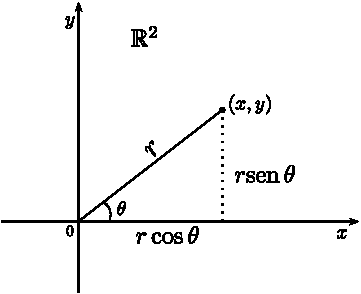
\includegraphics[scale=1.2]{Figuras/fig-coordenadas-polares}
\caption{A descrição em coordenadas polares de um número complexo $z=x+iy$.}
\label{fig-coord-polares}
\end{figure}

Daí segue que qualquer número complexo não-nulo $z=x+iy$ pode ser escrito como
$z=r(\cos\theta+i\sen\theta)$, onde $r=|z|=\sqrt{x^2+y^2}$. 
Esta é chamada de representação ou forma polar do número complexo $z$.
\index{Forma polar}
O ângulo $\theta$ da forma polar é chamado de \textit{um argumento} de $z$. 
Já que as funções seno e cosseno são funções periódicas de período $2\pi$ é 
natural pensar no angulo $\theta+2k\pi$, com $k\in\mathbb{Z}$, como 
também sendo um argumento de $z$. Para evitar este tipo de multiplicidade na determinação 
de um argumento é que restringimos acima as medidas de ângulos ao intervalo $[0,2\pi)$.
Desta maneira, cada número complexo não-nulo tem um argumento definido de forma única.
Mais a frente quando estivermos trabalhando com as funções exponencial e logaritmo 
complexo vamos discutir em detalhes o conceito de \textit{ramo do argumento}. 

Exemplificando, o número complexo $z=1+1i$ é identificado com o ponto $(1,1)\in\mathbb{R}^2$
que tem norma $\|(1,1)\|=\sqrt{2}$ e está localizado na bissetriz do primeiro quadrante 
sendo assim representado em coordenadas polares 
por $x=\sqrt{2}\cos(\pi/4)$ e $y=\sqrt{2}\sen(\pi/4)$.
Portanto a representação polar de $z=\sqrt{2}(\cos(\pi/4)+i\sen(\pi/4))$.


Vamos ver agora como fica a representação polar de um produto de dois números
complexos. Sejam $z,w\in\mathbb{C}$ cujas representações polares são dadas por
\begin{align*}
z = r(\cos\theta+i\sen\theta)\\
w = s(\cos\beta+i\sen\beta).
\end{align*}
Para obter a representação polar de $zw$ basta efetuar o produto destes dois números
em suas representações polares e usar as fórmulas bem conhecidas para seno e cosseno
da soma de dois ângulos como segue:
\begin{align}\label{eq-formula-prod-zw-coord-polares}
zw
&=
r(\cos\theta+i\sen\beta)s(\cos\beta+i\sen\beta)
\nonumber\\
&=
rs \big( (\cos\theta\cos\beta-\sen\theta\sen\beta) +i(\cos\theta\sen\beta+\sen\theta\cos\beta)\big)
\nonumber\\
&=
rs (\cos(\theta+\beta)+i\sen(\theta+\beta)).
\end{align}

É muito importante observar que $\theta+\beta$ não é necessariamente um argumento 
de $zw$, no sentido de que este ângulo pode estar fora do intervalo $[0,2\pi)$.
Isto poderia acontecer se os argumentos de $z$ e $w$ fossem, por exemplo, ambos
maiores que $\pi$. Veja o exemplo da figura abaixo:
\begin{figure}[h]
\centering
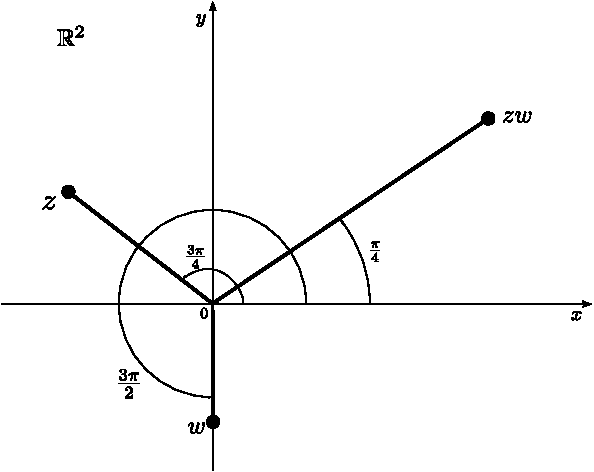
\includegraphics[scale=0.9]{Figuras/fig-prod-argumento}
\caption{Um argumento do produto $zw$}
\label{fig-coord-polares2}
\end{figure}

No exemplo da figura acima temos 
\begin{align*}
z=|z|(\cos(3\pi/4)+i\sen(3\pi/4))
\\[0.2cm]
w=|w|(\cos(3\pi/2)+i\sen(3\pi/2)).
\end{align*}
Aplicando a fórmula que deduzimos acima, ficamos com 
\[
zw=|z||w|(\cos(9\pi/4)+i\sen(9\pi/4)).
\]
Note que tudo está correto, mas como o ângulo que nossa fórmula para o produto fornece resulta em um valor 
maior que $2\pi$ quem de fato representará o argumento do produto $zw$, 
no intervalo anteriormente especificado $[0,2\pi)$, 
será o ângulo $\pi/4$, como mostrado na figura acima.

Este exemplo alerta para o fato de que, em geral, não é verdade que um argumento de um produto $zw$
é igual a soma dos argumentos de $z$ e $w$. Porém a menos de múltiplos inteiros de $2\pi$ isto 
é de fato verdadeiro. Mais a frente, quando apresentarmos a definição de ramo do argumento, 
de um número complexo $z$, que será denotado por $\mathrm{arg}(z)$, 
poderemos escrever esta última observação de modo mais sucinto através da notação abaixo
\[
\mathrm{arg}(zw) \equiv \mathrm{arg}(z)+\mathrm{arg}(w) \quad  (\mathrm{mod}\ 2\pi),
\] 
onde para qualquer $\alpha\in\mathbb{R}$ o símbolo $\alpha\ (\mathrm{mod}\ 2\pi)$
denota o único ângulo $\theta\in [0,2\pi)$ com a propriedade
que existe um único inteiro $k$ tal que $\theta +2k\pi= \alpha$.



Tomando $w=z$ em \eqref{eq-formula-prod-zw-coord-polares} obtemos
\[
z^2 = r^2(\cos(2\theta)+i\sen(2\theta)).
\] 
Esta igualdade sugere que as potencias sucessivas $z$ admite a seguinte representação
\[
z^n = r^n (\cos(n\theta)+i\sen(n\theta)), \quad \forall n\in\mathbb{N}.
\]
Esta afirmação é de fato verdadeira e pode ser facilmente obtida 
procedendo uma indução formal em $n$ e usando a identidade \eqref{eq-formula-prod-zw-coord-polares}.
Esta identidade é conhecida como Fórmula de De Moivre.
\index{Formula@Fórmula!De Moivre} 
Vamos usá-la no que segue para extrair 
raízes de um número complexo não-nulo arbitrário. 

Seja $w$ um número complexo não-nulo. Uma raíz $n$-ésima (ou de ordem $n$)
de $w$ é um número complexo $z$ satisfazendo a equação 
\[
z^n = w.
\]
Para procurar uma raíz $n$-ésima de $w$ vamos reescrever a equação acima 
usando coordenadas polares. Sejam $\beta\in [0,2\pi)$ um argumento de $w$ e $s=|w|$ 
a norma de $w$. Vamos escrever $z$ em coordenadas como $z=r(\cos\theta+i\sen\theta)$.
Pela Fórmula de De Moivre temos que $z^n=r^n(\cos(n\theta)+i\sen(n\theta))$.
Portanto 
\begin{align}\label{eq-aux-raiz-nesima-w}
z^n=w \quad \Longleftrightarrow \quad r^n(\cos(n\theta)+i\sen(n\theta)) = s(\cos\beta+i\sen\beta).
\end{align}
Tomando módulo dos dois lados da última igualdade acima, usando (I.7), $s>0$, $r\geqslant 0$ 
e que $|\cos\alpha+i\sen\alpha|=1$ para qualquer $\alpha\in\mathbb{R}$ temos que 
\begin{eqnarray*}
&|r^n(\cos(n\theta)+i\sen(n\theta))| = |s(\cos\beta+i\sen\beta)|&
\\[0.3cm]
&\Downarrow&
\\[0.3cm]
&r^n|\cos(n\theta)+i\sen(n\theta))| = s|(\cos\beta+i\sen\beta)|&
\\[0.3cm]
&\Downarrow&
\\[0.3cm]
&r^n=s.&
\end{eqnarray*}
Portanto $r = \sqrt[n]{s}$ e isto implica que qualquer solução $z$ da 
equação $z^n=w$ é tal que $|z|=  \sqrt[n]{s}$. Já que $s>0$ e $r^n=s$ podemos
concluir de \eqref{eq-aux-raiz-nesima-w} que o argumento $\theta$ de qualquer solução 
da equação satisfaz
$
\cos(n\theta)+i\sen(n\theta) = \cos\beta+i\sen\beta.
$
Já que dois números complexos são iguais se e somente se suas partes real e imaginária
coincidem, podemos afirmar que $\theta$ é solução do sistema não-linear
\[
\begin{cases}
\cos(n\theta)=\cos\beta
\\[0.1cm]
\sen(n\theta)=\sen(\beta).
\end{cases}
\]

Usando que as funções seno e cosseno são funções periódicas de período $2\pi$
concluímos que para cada $k\in\mathbb{Z}$ fixado o ângulo $\theta\equiv \theta(k,\beta)$ 
satisfazendo a igualdade $n\theta = \beta + 2k\pi$ é uma solução do sistema acima.
Para representar $z$ em coordenadas polares é preciso escolher dentre todas estas 
soluções apenas aquelas que satisfazem a condição $\theta\in [0,2\pi)$.
Desta forma só nos interessa os valores de $k$ para os quais 
temos 
\begin{align}\label{eq-aux2-raiz-nesima-w}
0\leqslant \frac{\beta}{n}+ \frac{2k\pi}{n}<2\pi. 
\end{align}
Lembrando que $\beta\in [0,2\pi)$ temos que 
\begin{align}\label{eq-aux3-raiz-nesima-w}
0\leqslant \frac{\beta}{n}<\frac{2\pi}{n}.
\end{align}
Usando a primeira desigualdade que aparece em \eqref{eq-aux2-raiz-nesima-w} e em seguida
a segunda desigualdade em \eqref{eq-aux3-raiz-nesima-w} obtemos a seguinte as seguintes desigualdades
\[
-\frac{2\pi k}{n}\leqslant \frac{\beta}{n}<\frac{2\pi}{n}
\quad \Longrightarrow \quad 
-\frac{2\pi k}{n}<\frac{2\pi}{n}
\quad \Longrightarrow \quad
\quad -k<1\quad 
\Longrightarrow \quad 
k>-1.
\]
Já que $k$ tem que ser um número inteiro então $k$ deve ser escolhido de forma que 
$k\geqslant 0$. 

Usando agora a segunda desigualdade em \eqref{eq-aux2-raiz-nesima-w} e a primeira 
desigualdade em \eqref{eq-aux3-raiz-nesima-w} temos que 
\[
\frac{\beta}{n}+ \frac{2k\pi}{n}<2\pi
\quad \Longrightarrow \quad 
\frac{2k\pi}{n}<2\pi-\frac{\beta}{n}
<
2\pi
\quad \Longrightarrow \quad 
2k\pi<2n\pi
\quad \Longrightarrow \quad 
k<n.
\]
Juntando esta restrição com a anterior podemos ver que devemos escolher $k\in \{0,1,2,\ldots,n-1\}$.


Desta forma cada um dos números complexos 
\begin{align}\label{eq-sol-ZN=w}
z_k = 
\sqrt[n]{s}
	\left(
		\cos\Big(\frac{\beta}{n}+ \frac{2k\pi}{n}\Big)+i\sen\Big(\frac{\beta}{n}+ \frac{2k\pi}{n}\Big)
	\right),
	\qquad 0\leqslant k\leqslant n-1
\end{align}
é uma solução de $z^n=w$. Como esta equação admite no máximo $n$ soluções e a lista acima 
possui exatamente $n$ elementos concluímos finalmente que os 
números $\{z_0,z_1,\ldots, z_{n-1}\}$ são todas as soluções possíveis desta equação. 


Um caso particular muito importante é o caso em que $w=1$. Neste caso as soluções da equação 
$z^n=1$ são chamadas de raízes $n$-ésimas da unidade. 
\index{Raízes da unidade}
Para $w=1$, temos $s=1$ e $\beta=0$. 
Logo fórmula das raízes $n$-ésimas obtida acima se reduz a 
\[
z_k = 
		\cos\Big(\frac{2k\pi}{n}\Big)+i\sen\Big(\frac{2k\pi}{n}\Big),
	\qquad 0\leqslant k\leqslant n-1.
\]
Este conjunto é chamado do conjunto das raízes $n$-ésimas da unidade. 
Ele pode ser também descrito, graças a Fórmula de De Moivre, 
de uma maneira ainda mais sucinta, isto é, como um conjunto de potências
sucessivas do número complexo 
$\omega = z_1 = $
isto é, $\{1,\omega,\omega^{2},\ldots,\omega^{n-1}\}$.


A título de exemplo vamos calcular as raízes cúbicas e quarta da unidade. 
Primeiro as raízes cúbicas da unidade. 
Usando a fórmula deduzida acima temos que as raízes cúbicas da unidade
são dadas por $\{1,\omega,\omega^2\}$, onde 
\[
\omega 
= 
\cos\Big(\frac{2\pi}{3}\Big)+i\sen\Big(\frac{2\pi}{3}\Big)
=
-\frac{1}{2}+i\frac{\sqrt{3}}{2}
\]
e pela Fórmula de De Moivre 
\[
\omega^2
= 
\cos\Big(\frac{4\pi}{3}\Big)+i\sen\Big(\frac{4\pi}{3}\Big)
=
-\frac{1}{2}-i\frac{\sqrt{3}}{2}.
\]

Para calcular as raízes quartas da unidade basta proceder como acima, mas 
observando que agora o conjunto é dado por $\{1,\omega,\omega^2,\omega^3\}$,
com $\omega$ neste caso dado por 
\[
\omega 
= 
\cos\Big(\frac{2\pi}{4}\Big)+i\sen\Big(\frac{2\pi}{4}\Big)
=
i.
\]
Logo $\omega^2 = i^2 =-1$ e $\omega^{3}=-i$.

\begin{figure}[h]
\centering
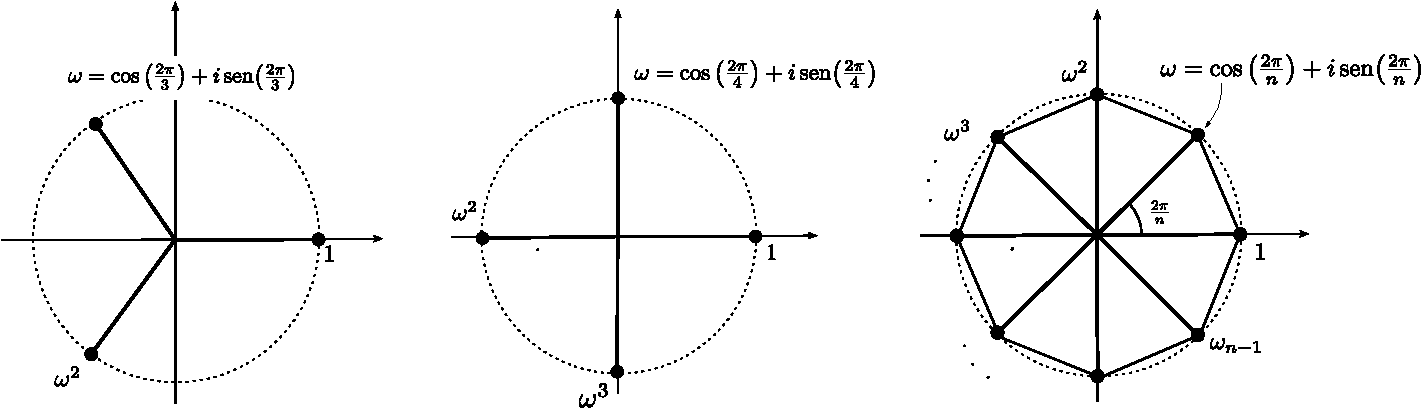
\includegraphics[scale=0.6]{Figuras/raizes-da-unidade}
\caption{Primeira figura representa as raízes cúbicas da unidade, a segunda as raízes quartas da unidade, e a última
o caso geral das raízes $n$-ésimas da unidade.}
\label{fig-raizes-unidade}
\end{figure}

\break 

Para finalizar esta seção observamos que as raízes $n$-ésimas da unidade 
determina o conjunto de vértices de um polígono regular $n$ lados inscrito 
no círculo de centro zero e raio um, como mostrado na Figura \ref{fig-raizes-unidade}.

%%%% Para escrever os apendices basta usar os comandos abaixo.
\begin{subappendices}
\markboth{Ap\^{e}ndice 1}{Ap\^{e}ndice 1}

Esta seção é baseada em um dos volumes da fantástica coleção de livros de Análise 
escritas por Barry Simon. Fora o exemplo que é totalmente desenvolvido aqui 
as demais informações seguem de perto a exposição de Barry Simon e
podem ser encontradas no Capítulo 1 da referência \cite{MR3443339}.



\section{Observações Históricas}
O uso de expressões como ``imaginário'' e ``complexo'' atestam que o processo de aceitação 
dos números complexos foi bastante difícil. Podemos pensar que, 
dada a fórmula para soluções da equação quadrática, que raízes quadradas 
de números negativos tivessem um passado muito antigo. 
Muitos imaginam que a motivação para se introduzir números complexos
tenha vindo de tempos antigos e de pessoas 
que se sentiam desconfortáveis com o fato de equações como $x^2+1=0$ 
não ter solução. A verdade é que os números complexo vieram mesmo do estudo 
de equações cúbicas, da forma 
\[
x^3-ax-b=0.
\]
Em 1515, Scipione del Ferro (1465-1526) deduziu que 
\begin{align}\label{formula-del-Ferro}
x
=
\sqrt[3]{ \frac{b}{2} +  \sqrt[2]{ \frac{b^2}{4}-\frac{a^3}{27} }  }
+
\sqrt[3]{ \frac{b}{2} -  \sqrt[2]{ \frac{b^2}{4}-\frac{a^3}{27} }  }
\end{align}
era uma solução desta cúbica, mas nunca publicou sua descoberta.
O mais intrigante e que mesmo em casos onde 
\begin{align}\label{eq-aux1-del-Ferro} 
\frac{b^2}{4}-\frac{a^3}{27}<0
\end{align}
a solução de del Ferro fornecia, depois de simplificada, um número real como solução da cúbica!

Um caso muito particular mas que ilustra bem como deve ter sido desafiante para del Ferro 
entender o que estava acontecendo é o caso em que tomamos $b=2$ e $a=3\sqrt[3]{2}$.
Estes valores foram escolhidos para fazer com que a expressão do lado esquerdo da desigualdade \eqref{eq-aux1-del-Ferro}
seja exatamente $-1$ e portanto
\[
x =
\sqrt[3]{1+\sqrt[2]{(-1)}}
+
\sqrt[3]{1-\sqrt[2]{(-1)}}
\]
O que obviamente era uma expressão que del Ferro, na época, deveria considerar muito intrigante,
principalmente porque o número $x$ que aparece acima (apesar desta representação complexa) 
é na realidade um número real! Vamos provar este 
fato abaixo, porém, usando ferramentas do século XX.

Primeiro precisamos fazer uma escolha para $\sqrt[2]{(-1)}$. A escolha mais 
natural hoje em dia é definir este número como sendo uma das duas soluções distintas da equação $z^2=-1$. 
Na seção anterior vimos como calcular as raízes desta equação e que elas são dadas por 
$z=i$ e $z=-i$.
A simetria presente na expressão de del Ferro fará com que o valor $x$ seja o mesmo para qualquer uma 
das duas escolhas $\sqrt[2]{(-1)}=i$ 
ou $\sqrt[2]{(-1)}=-i$.
Por simplicidade vamos tomar $\sqrt{(-1)}=i$. Substituindo na expressão acima 
ficamos com 
\[
x =
\sqrt[3]{1+i}
+
\sqrt[3]{1-i}.
\]
Raciocinando de maneira análoga, podemos definir $\sqrt[3]{1+i}$ 
como sendo (na notação da seção anterior) a solução $z_0$ da equação $z^3=1+i$. 
Para isto basta escrever $1+i$ em coordenadas polares $1+i = \sqrt{2}(\cos\pi/4+i\sen\pi/4)$
e usar a fórmula dada para $z_0$, obtendo a seguinte expressão:
\[
\sqrt[3]{1+i} = (\sqrt{2})^{\frac{1}{3}}\Big(\cos\big(\frac{\pi}{12}\big)+i\sen\big(\frac{\pi}{12})\Big)
\]
Repetimos o mesmo procedimento para $\sqrt[3]{1-i}$. 
Novamente, para encontrar a solução $z_0$ da equação $z^3=1-i$ primeiro escrevemos $1-i$ em coordenadas polares
$1-i = \sqrt{2}\big(\cos(7\pi/4) +i\sen(7\pi/4)\big)$. Depois aplicamos a fórmula para $z_0$ e temos
que 
\[
\sqrt[3]{1-i} = (\sqrt{2})^{\frac{1}{3}}\Big(\cos\big(\frac{7\pi}{12}\big)+i\sen\big(\frac{7\pi}{12})\Big).
\]

Já que os senos que aparecem nas duas expressões em destaque acima, quando somados, 
se anulam e os cossenos têm o mesmo valor descobrimos que 
\[
x= 
2\sqrt[6]{2}\cos\big(\frac{\pi}{12}\big) 
= 
2\sqrt[6]{2}\cdot \frac{1+\sqrt{3}}{2\sqrt{2}}
=
\frac{1+\sqrt{3}}{\sqrt[3]{2}}.
\]

Com esta raíz em mãos é simples descobrir quais são as outras duas, basta 
aplicar o algoritmo da divisão de polinômios e em seguida a Fórmula de Bhaskara. 
Feito isto descobrimos que todas as suas raízes são reais e dadas por
\[
x= \frac{1+\sqrt{3}}{\sqrt[3]{2}},\quad 
x= -\sqrt[3]{4} \quad \text{e}\quad x= \frac{1-\sqrt{3}}{\sqrt[3]{2}}.
\]

A fórmula de del Ferro \eqref{formula-del-Ferro} foi publicada em um livro de Girolamo Cardano (1501-1576) em 1545.
Apesar do livro de Cardano ter exemplos onde $b^2/4-a^3/27<0$ ele nunca aplicou 
a fórmula neste casos!


Vinte e sete anos mais tarde, Rafael Bombelli (1526-1572) publicou um livro
que continha instruções do que viria a ser no futuro as regras da aritmética no 
conjunto dos números complexo e as usou para encontrar raízes reais de cúbicas
a partir da fórmula de del Ferro. A publicação chave para deslanchar a teoria
dos números complexos foi o trabalho de Wallis e Euler que apareceram por volta de 1748.
Em particular, nesta época Euler esclarece como deveriam ser entendidas as raízes da unidade.
Usando suas técnicas ele mostra que \eqref{formula-del-Ferro} 
era uma fórmula que na verdade representa não apenas uma, mas em diversos casos 
várias das raízes da cúbica. Mesmo após estas grandes descobertas ainda foram necessários
mais cem anos para a comunidade matemática aceitar completamente os números complexos.
Assim muito do trabalho de Cauchy (que é um dos pais fundadores da teria do cálculo integral e diferencial
de funções complexas) foi realizado em uma atmosfera em que mesmo o próprio Cauchy não se sentia muito 
confortável. 

O ponto de vista geométrico dos números complexos, como pontos do plano Euclidiano, 
foi introduzido por Jean-Robert Argand(1768-1822) e Caspar Wessel (1745-1818) e defendida
por Gauss. Argand e Wessel não eram matemáticos profissionais. Wessel era um agrimensor
e apresentou sua interpretação geométrica para a Acadêmia Real Dinamarquesa em 1797.
Em seguida, em 1799 seu trabalho foi publicado e pouco depois esquecido e não teve
nenhum impacto. Mais tarde a abordagem geométrica foi redesenvolvida por 
dois matemáticos dinamarqueses Sophus Christian Juel e o famoso Sophus Lie.

Argand era um contador e livreiro, e em 1806 publicou por conta própria seu 
trabalho em um livro que apareceu sem o seu nome! Em 1813 um matemático Francês,
Jacques Français, publicou um artigo que dava sequência ao trabalho de Argand,
onde ele solicitou que o autor do misterioso livro se revelasse. Desta forma 
Argand recebeu reconhecimento por seu trabalho e figuras 
geométricas como as da Figura \ref{fig-coord-polares} são frequentemente chamadas de diagramas
de Argand. 



\end{subappendices}
